\documentclass[12pt, letterpaper]{article}
\usepackage[margin=1in]{geometry}
\usepackage{tikz}
\usepackage{pgfplots}
\pgfplotsset{compat=1.18}
\usetikzlibrary{arrows.meta, shapes.geometric, shapes.multipart, positioning,
    fit, backgrounds, decorations.pathreplacing, calc, matrix}
\usepackage{xcolor}
\usepackage{booktabs}
\usepackage{array}
\usepackage{multicol}
\usepackage{tcolorbox}
\tcbuselibrary{skins, breakable}
\usepackage{fancyhdr}
\usepackage{titlesec}
\usepackage{enumitem}
\usepackage{amsmath}
\usepackage{amssymb}
% \usepackage{fontawesome5}  % Uncomment if fontawesome5 is installed

% ---- Colors ----
\definecolor{accentblue}{RGB}{31,73,125}
\definecolor{dangerred}{RGB}{192,0,0}
\definecolor{safegreen}{RGB}{0,120,0}
\definecolor{warnyellow}{RGB}{200,130,0}
\definecolor{lightblue}{RGB}{220,235,252}
\definecolor{lightred}{RGB}{252,220,220}
\definecolor{lightgreen}{RGB}{210,240,210}
\definecolor{lightyellow}{RGB}{255,245,210}
\definecolor{slategray}{RGB}{112,128,144}

% ---- Page style ----
\pagestyle{fancy}
\fancyhf{}
\fancyhead[L]{\small\textbf{\color{accentblue}Agentic AI Bootcamp} \textbar\ Evaluating Safety \& Performance}
\fancyhead[R]{\small Army Cyber Institute, USMA}
\fancyfoot[C]{\small\thepage}
\renewcommand{\headrulewidth}{1.5pt}
\renewcommand{\headrule}{\hbox to\headwidth{\color{accentblue}\leaders\hrule height \headrulewidth\hfill}}

% ---- Section formatting ----
\titleformat{\section}{\large\bfseries\color{accentblue}}{}{0em}{}[\titlerule]
\titleformat{\subsection}{\normalsize\bfseries\color{slategray}}{}{0em}{}

% ---- tcolorbox styles ----
\tcbset{
    safetybox/.style={colback=lightred, colframe=dangerred, fonttitle=\bfseries\small, title style={fill=dangerred}},
    perfbox/.style={colback=lightblue, colframe=accentblue, fonttitle=\bfseries\small, title style={fill=accentblue}},
    notebox/.style={colback=lightyellow, colframe=warnyellow, fonttitle=\bfseries\small}
}

\begin{document}

\begin{center}
    {\LARGE\bfseries\color{accentblue} Agentic AI: Safety \& Performance Evaluation}\\[4pt]
    {\large Teaching Reference Sheet --- Diagrams, Metrics, and Quick Reference}\\[2pt]
    {\small Army Cyber Institute $\cdot$ U.S. Military Academy $\cdot$ Agentic AI Bootcamp}
    \vspace{0.3cm}
    \hrule height 2pt
    \vspace{0.1cm}
    \hrule height 0.5pt
\end{center}

% ============================================================
\section{Diagram 1: Undesired LLM Behavior Taxonomy}
% ============================================================

\begin{center}
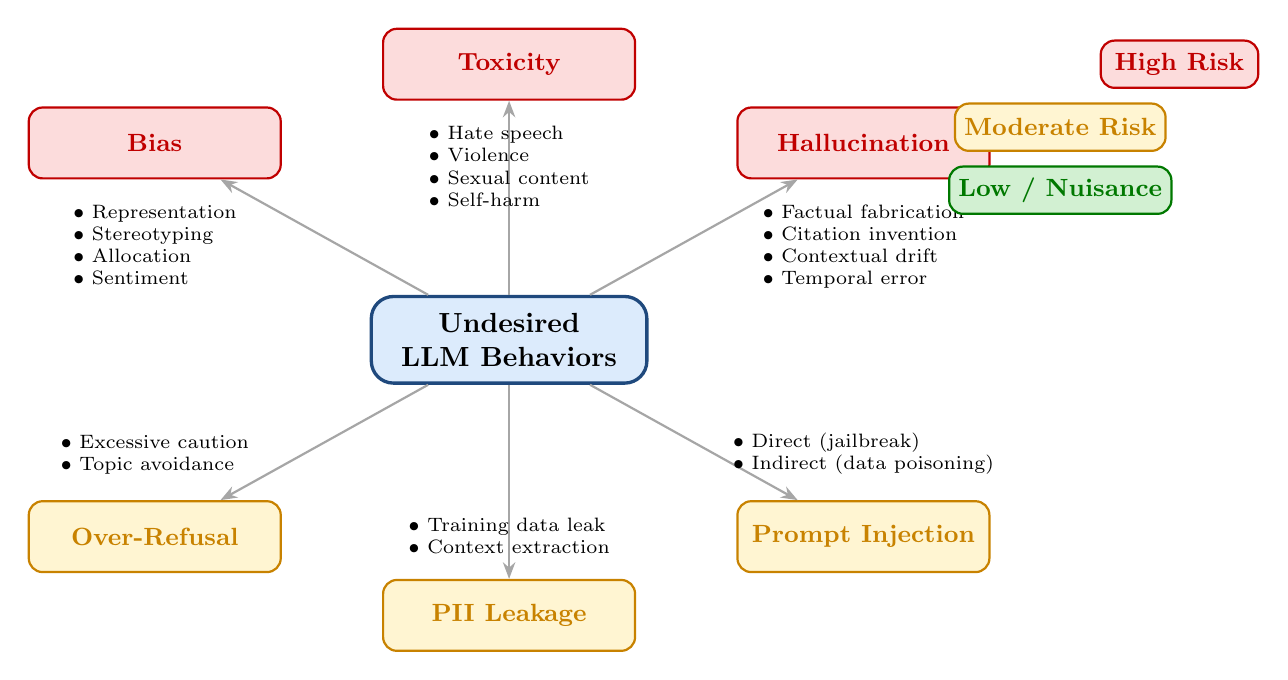
\begin{tikzpicture}[
    scale=1.0,
    mainbox/.style={rectangle, rounded corners=8pt, draw=accentblue, very thick, fill=lightblue,
        minimum width=3.5cm, minimum height=1.1cm, align=center, font=\bfseries},
    highbox/.style={rectangle, rounded corners=5pt, draw=dangerred, thick, fill=lightred,
        minimum width=3.2cm, minimum height=0.9cm, align=center, font=\small\bfseries, text=dangerred},
    modbox/.style={rectangle, rounded corners=5pt, draw=warnyellow, thick, fill=lightyellow,
        minimum width=3.2cm, minimum height=0.9cm, align=center, font=\small\bfseries, text=warnyellow},
    lowbox/.style={rectangle, rounded corners=5pt, draw=safegreen, thick, fill=lightgreen,
        minimum width=3.2cm, minimum height=0.9cm, align=center, font=\small\bfseries, text=safegreen},
    arrow/.style={-{Stealth[length=6pt]}, thick}
]
    % Center
    \node[mainbox] (center) at (0,0) {Undesired\\LLM Behaviors};

    % High risk
    \node[highbox] (bias)    at (-4.5,  2.5) {Bias};
    \node[highbox] (toxic)   at (0,     3.5) {Toxicity};
    \node[highbox] (halluc)  at (4.5,   2.5) {Hallucination};

    % Moderate risk
    \node[modbox]  (inject)  at (4.5,  -2.5) {Prompt Injection};
    \node[modbox]  (pii)     at (0,    -3.5) {PII Leakage};
    \node[modbox]  (refusal) at (-4.5, -2.5) {Over-Refusal};

    % Arrows
    \foreach \n in {bias, toxic, halluc, inject, pii, refusal}
        \draw[arrow, gray!70] (center) -- (\n);

    % Sub-bullets
    \node[font=\scriptsize, align=left, below=0.2cm of bias] {%
        $\bullet$ Representation\\
        $\bullet$ Stereotyping\\
        $\bullet$ Allocation\\
        $\bullet$ Sentiment};

    \node[font=\scriptsize, align=left, below=0.2cm of toxic] {%
        $\bullet$ Hate speech\\
        $\bullet$ Violence\\
        $\bullet$ Sexual content\\
        $\bullet$ Self-harm};

    \node[font=\scriptsize, align=left, below=0.2cm of halluc] {%
        $\bullet$ Factual fabrication\\
        $\bullet$ Citation invention\\
        $\bullet$ Contextual drift\\
        $\bullet$ Temporal error};

    \node[font=\scriptsize, align=left, above=0.2cm of inject] {%
        $\bullet$ Direct (jailbreak)\\
        $\bullet$ Indirect (data poisoning)};

    \node[font=\scriptsize, align=left, above=0.2cm of pii] {%
        $\bullet$ Training data leak\\
        $\bullet$ Context extraction};

    \node[font=\scriptsize, align=left, above=0.2cm of refusal] {%
        $\bullet$ Excessive caution\\
        $\bullet$ Topic avoidance};

    % Legend
    \node[highbox, minimum width=2cm, minimum height=0.6cm, right=0.5cm of toxic] at (7, 3.5) {High Risk};
    \node[modbox,  minimum width=2cm, minimum height=0.6cm] at (7, 2.7) {Moderate Risk};
    \node[lowbox,  minimum width=2cm, minimum height=0.6cm] at (7, 1.9) {Low / Nuisance};

\end{tikzpicture}
\end{center}

\vspace{0.4cm}

% ============================================================
\section{Diagram 2: Multi-Layer Guardrail Architecture}
% ============================================================

\begin{center}
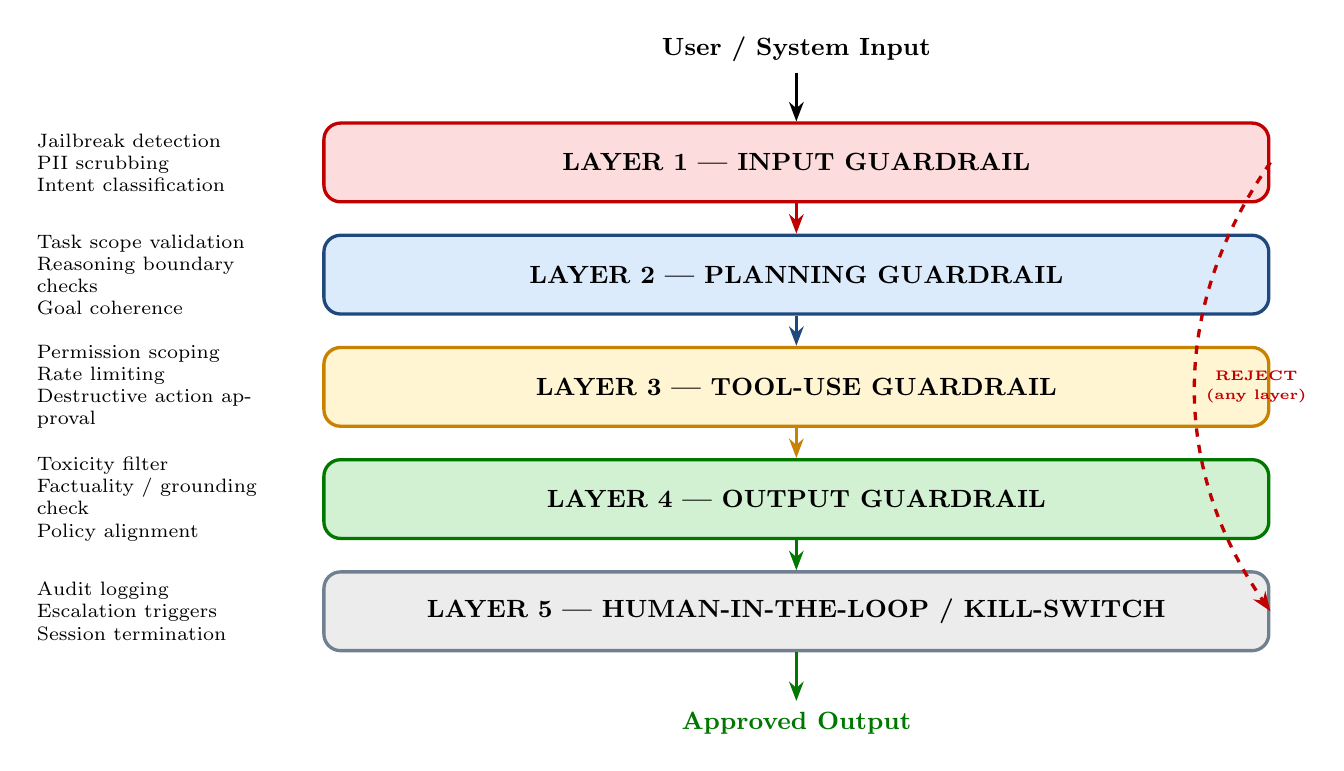
\begin{tikzpicture}[scale=0.95,
    layer/.style={rectangle, rounded corners=6pt, draw, very thick, minimum width=12cm, minimum height=1.0cm, align=center, font=\small\bfseries},
    arrow/.style={-{Stealth[length=7pt]}, very thick},
    sidenote/.style={font=\scriptsize, align=left, text width=3cm}
]
    % Layers
    \node[layer, fill=lightred, draw=dangerred]        (L1) at (0, 5.0)
        {LAYER 1 --- INPUT GUARDRAIL};
    \node[layer, fill=lightblue, draw=accentblue]      (L2) at (0, 3.5)
        {LAYER 2 --- PLANNING GUARDRAIL};
    \node[layer, fill=lightyellow, draw=warnyellow]    (L3) at (0, 2.0)
        {LAYER 3 --- TOOL-USE GUARDRAIL};
    \node[layer, fill=lightgreen, draw=safegreen]      (L4) at (0, 0.5)
        {LAYER 4 --- OUTPUT GUARDRAIL};
    \node[layer, fill=gray!15, draw=slategray]         (L5) at (0,-1.0)
        {LAYER 5 --- HUMAN-IN-THE-LOOP / KILL-SWITCH};

    % Down arrows
    \draw[arrow, dangerred]  (L1) -- (L2);
    \draw[arrow, accentblue] (L2) -- (L3);
    \draw[arrow, warnyellow] (L3) -- (L4);
    \draw[arrow, safegreen]  (L4) -- (L5);

    % Reject bypass arrow
    \draw[arrow, dashed, dangerred, bend right=35]
        (L1.east) to node[right, font=\tiny\bfseries, color=dangerred]{\shortstack{REJECT\\(any layer)}} (L5.east);

    % Side annotations (left)
    \node[sidenote, left=0.5cm of L1] {Jailbreak detection\\PII scrubbing\\Intent classification};
    \node[sidenote, left=0.5cm of L2] {Task scope validation\\Reasoning boundary checks\\Goal coherence};
    \node[sidenote, left=0.5cm of L3] {Permission scoping\\Rate limiting\\Destructive action approval};
    \node[sidenote, left=0.5cm of L4] {Toxicity filter\\Factuality / grounding check\\Policy alignment};
    \node[sidenote, left=0.5cm of L5] {Audit logging\\Escalation triggers\\Session termination};

    % Input arrow at top
    \draw[arrow, very thick, black] (0, 6.2) -- (L1.north) node[above, font=\small\bfseries, pos=0]{User / System Input};

    % Output arrow at bottom
    \draw[arrow, very thick, safegreen] (L5.south) -- (0,-2.2) node[below, font=\small\bfseries, pos=1]{Approved Output};
\end{tikzpicture}
\end{center}

\newpage

% ============================================================
\section{Diagram 3: Latency Budget Breakdown}
% ============================================================

\begin{center}
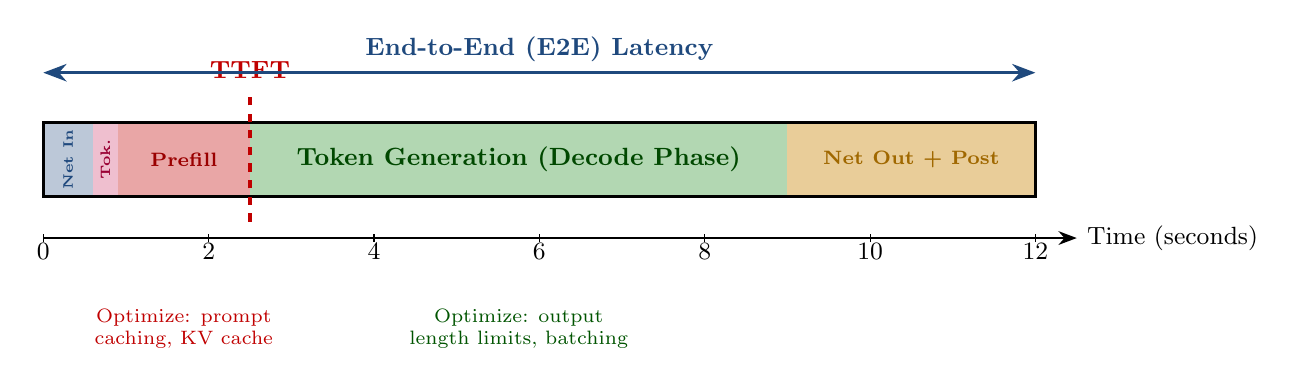
\begin{tikzpicture}[scale=1.05]
    % Segments
    \fill[accentblue!30]  (0,0)   rectangle (0.6,0.9);
    \fill[purple!25]      (0.6,0) rectangle (0.9,0.9);
    \fill[dangerred!35]   (0.9,0) rectangle (2.5,0.9);
    \fill[safegreen!30]   (2.5,0) rectangle (9.0,0.9);
    \fill[warnyellow!40]  (9.0,0) rectangle (12,0.9);

    % Border
    \draw[very thick] (0,0) rectangle (12,0.9);

    % TTFT marker
    \draw[dangerred, very thick, dashed] (2.5,-0.3) -- (2.5,1.3)
        node[above, font=\small\bfseries, color=dangerred] {TTFT};

    % Segment labels inside bars
    \node[font=\tiny\bfseries, rotate=90, text=accentblue] at (0.3, 0.45) {Net In};
    \node[font=\tiny\bfseries, rotate=90, text=purple!80!black] at (0.75, 0.45) {Tok.};
    \node[font=\scriptsize\bfseries, text=dangerred!80!black] at (1.7, 0.45) {Prefill};
    \node[font=\small\bfseries, text=safegreen!60!black] at (5.75, 0.45) {Token Generation (Decode Phase)};
    \node[font=\scriptsize\bfseries, text=warnyellow!80!black] at (10.5, 0.45) {Net Out + Post};

    % Time axis
    \draw[-{Stealth}, thick] (0,-0.5) -- (12.5,-0.5) node[right, font=\small]{Time (seconds)};
    \foreach \x/\t in {0/0, 2/2, 4/4, 6/6, 8/8, 10/10, 12/12}
        \draw (\x,-0.55) -- (\x,-0.45) node[below, font=\small]{\t};

    % E2E bracket
    \draw[{Stealth}-{Stealth}, very thick, accentblue] (0, 1.5) -- (12, 1.5)
        node[midway, above, font=\small\bfseries, color=accentblue]{End-to-End (E2E) Latency};

    % Optimization hints
    \node[font=\scriptsize, align=center, text=dangerred, below=1.3cm of {(1.7,0)}] {Optimize: prompt\\caching, KV cache};
    \node[font=\scriptsize, align=center, text=safegreen!70!black, below=1.3cm of {(5.75,0)}] {Optimize: output\\length limits, batching};
\end{tikzpicture}
\end{center}

\vspace{0.5cm}

% ============================================================
\section{Diagram 4: Agentic Task Evaluation Flow}
% ============================================================

\begin{center}
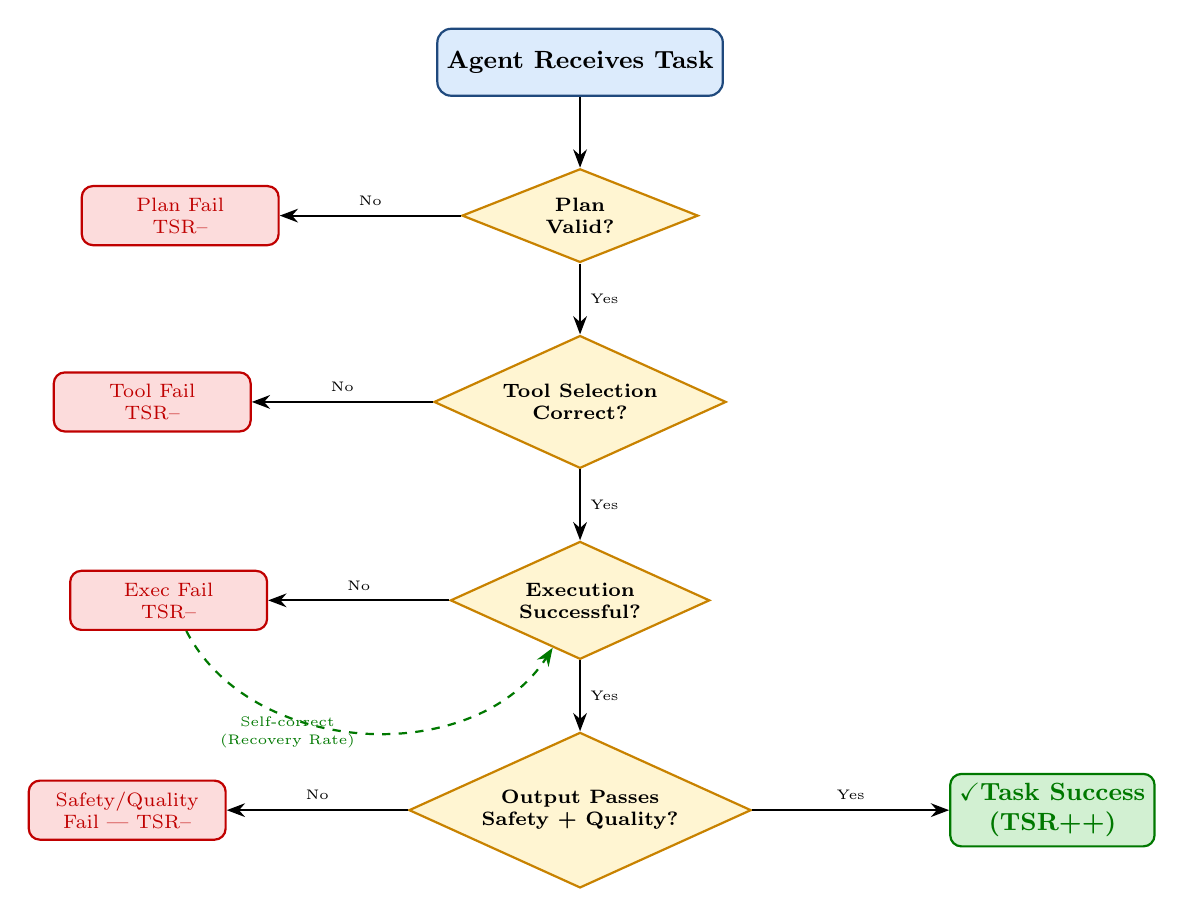
\begin{tikzpicture}[
    node distance=1.3cm and 2.5cm,
    block/.style={rectangle, rounded corners=5pt, draw=accentblue, thick, fill=lightblue,
        minimum width=3.2cm, minimum height=0.85cm, align=center, font=\small\bfseries},
    decide/.style={diamond, draw=warnyellow, thick, fill=lightyellow, aspect=2.2,
        align=center, font=\scriptsize\bfseries, minimum width=3cm, minimum height=0.6cm},
    failbox/.style={rectangle, rounded corners=4pt, draw=dangerred, thick, fill=lightred,
        minimum width=2.5cm, minimum height=0.75cm, align=center, font=\scriptsize, text=dangerred},
    okbox/.style={rectangle, rounded corners=4pt, draw=safegreen, thick, fill=lightgreen,
        minimum width=2.5cm, minimum height=0.75cm, align=center, font=\small\bfseries, text=safegreen},
    arrow/.style={-{Stealth}, thick}
]
    \node[block]  (task)   {Agent Receives Task};
    \node[decide, below=0.9cm of task]   (plan)   {Plan\\Valid?};
    \node[decide, below=0.9cm of plan]   (tools)  {Tool Selection\\Correct?};
    \node[decide, below=0.9cm of tools]  (exec)   {Execution\\Successful?};
    \node[decide, below=0.9cm of exec]   (output) {Output Passes\\Safety + Quality?};
    \node[okbox,  right=2.5cm of output] (success) {\checkmark Task Success\\(TSR++)};
    \node[failbox, left=2.3cm of plan]   (f1) {Plan Fail\\TSR--};
    \node[failbox, left=2.3cm of tools]  (f2) {Tool Fail\\TSR--};
    \node[failbox, left=2.3cm of exec]   (f3) {Exec Fail\\TSR--};
    \node[failbox, left=2.3cm of output] (f4) {Safety/Quality\\Fail --- TSR--};

    \draw[arrow] (task) -- (plan);
    \draw[arrow] (plan) -- node[right, font=\tiny]{Yes} (tools);
    \draw[arrow] (tools) -- node[right, font=\tiny]{Yes} (exec);
    \draw[arrow] (exec) -- node[right, font=\tiny]{Yes} (output);
    \draw[arrow] (output) -- node[above, font=\tiny]{Yes} (success);
    \draw[arrow] (plan)   -- node[above, font=\tiny]{No}  (f1);
    \draw[arrow] (tools)  -- node[above, font=\tiny]{No}  (f2);
    \draw[arrow] (exec)   -- node[above, font=\tiny]{No}  (f3);
    \draw[arrow] (output) -- node[above, font=\tiny]{No}  (f4);

    % Recovery loop
    \draw[arrow, dashed, safegreen, bend right=60]
        (f3) to node[left, font=\tiny, color=safegreen]{\shortstack{Self-correct\\(Recovery Rate)}} (exec);
\end{tikzpicture}
\end{center}

\newpage

% ============================================================
\section{Quick Reference: Key Metrics}
% ============================================================

\begin{multicols}{2}

\begin{tcolorbox}[safetybox, title={Safety Metrics Quick Reference}]
    \begin{tabular}{@{}p{2.5cm}p{4cm}@{}}
        \textbf{Metric} & \textbf{Description / Tool} \\
        \midrule
        Toxicity Score & Detoxify / Perspective API \\
        Bias Score & StereoSet, BBQ, WinoBias \\
        Faithfulness & RAGAS (RAG systems) \\
        TruthfulQA \% & LLM factuality benchmark \\
        Injection Rate & \% of injection attempts that succeed \\
        Policy Violation Rate & \% outputs flagged by guardrail \\
    \end{tabular}
\end{tcolorbox}

\vspace{0.3cm}

\begin{tcolorbox}[perfbox, title={Infrastructure Performance}]
    \begin{tabular}{@{}p{2.2cm}p{4cm}@{}}
        \textbf{Metric} & \textbf{Definition} \\
        \midrule
        TTFT & Time to first generated token \\
        E2E Latency & Full response wall-clock time \\
        TPS & Tokens per second (decode) \\
        P95 Latency & 95th percentile response time \\
        Cost/Task & (In tokens $\times$ rate) + (Out $\times$ rate) \\
        Context \% & Tokens used / context window \\
    \end{tabular}
\end{tcolorbox}

\columnbreak

\begin{tcolorbox}[perfbox, title={Agentic Task Performance}]
    \begin{tabular}{@{}p{2.4cm}p{4cm}@{}}
        \textbf{Metric} & \textbf{Formula / Definition} \\
        \midrule
        TSR & \% tasks fully completed \\
        GSR & \% sessions all sub-goals met \\
        Tool Accuracy & Correct tool / total selections \\
        Step Efficiency & Optimal steps / Actual steps \\
        Recovery Rate & \% errors self-corrected \\
        AVM & Value generated / Inference cost \\
    \end{tabular}
\end{tcolorbox}

\vspace{0.3cm}

\begin{tcolorbox}[notebox, title={AVM Formula}]
\[
    \text{AVM} = \frac{\text{Quantified Value (hrs, \$, errors avoided)}}{\text{Total Inference + Ops Cost}}
\]
    AVM $<$ 1: Net liability \quad AVM $>$ 3: Strong ROI
\end{tcolorbox}

\end{multicols}

% ============================================================
\section{Quick Reference: Tool Selection Guide}
% ============================================================

\begin{center}
\begin{tabular}{@{}p{3.5cm}p{4cm}p{4cm}p{2.5cm}@{}}
    \toprule
    \textbf{Problem} & \textbf{Best Tool(s)} & \textbf{Notes} & \textbf{Open Source?} \\
    \midrule
    Toxicity detection & Detoxify, Perspective API & Detoxify = local; Perspective = API & \checkmark / Partial \\
    Bias evaluation & StereoSet, BBQ, WinoBias & Use multiple benchmarks & \checkmark \\
    Hallucination (RAG) & RAGAS, FActScorer & RAGAS is easiest to integrate & \checkmark \\
    General factuality & TruthfulQA, HELM & HELM = comprehensive & \checkmark \\
    Jailbreak defense & LlamaGuard, NeMo & Air-gap safe & \checkmark \\
    Enterprise guardrails & Azure Content Safety, Bedrock & Managed, SLA-backed & \texttimes \\
    PII detection & Presidio (Microsoft) & Rule-based + ML hybrid & \checkmark \\
    Red teaming & PyRIT, Garak, Promptfoo & Automated adversarial probing & \checkmark \\
    Agent task eval & GAIA, SWE-bench, AgentBench & Multi-env benchmarks & \checkmark \\
    Holistic model eval & HELM & Stanford CRFM & \checkmark \\
    LLM-as-Judge & DeepEval, LangSmith, OpenAI Evals & Requires judge calibration & Partial \\
    \bottomrule
\end{tabular}
\end{center}

% ============================================================
\section{Diagram 5: Evaluation Pipeline Overview}
% ============================================================

\begin{center}
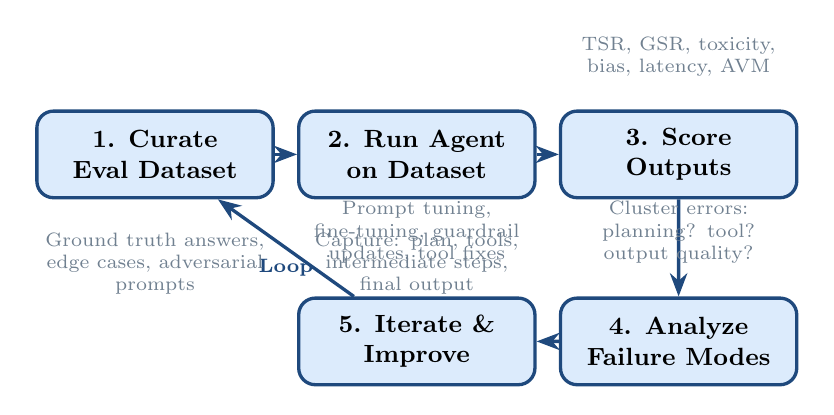
\begin{tikzpicture}[scale=0.95,
    pstep/.style={rectangle, rounded corners=6pt, draw=accentblue, very thick, fill=lightblue,
        minimum width=3.0cm, minimum height=1.1cm, align=center, font=\small\bfseries},
    arrow/.style={-{Stealth}, very thick, accentblue},
    annot/.style={font=\scriptsize, align=center, text width=3cm, text=slategray}
]
    \node[pstep] (data)    at (0,   0) {1. Curate\\Eval Dataset};
    \node[pstep] (run)     at (3.5, 0) {2. Run Agent\\on Dataset};
    \node[pstep] (score)   at (7.0, 0) {3. Score\\Outputs};
    \node[pstep] (analyze) at (7.0,-2.5) {4. Analyze\\Failure Modes};
    \node[pstep] (improve) at (3.5,-2.5) {5. Iterate \&\\Improve};

    \draw[arrow] (data)    -- (run);
    \draw[arrow] (run)     -- (score);
    \draw[arrow] (score)   -- (analyze);
    \draw[arrow] (analyze) -- (improve);
    \draw[arrow, bend right=0] (improve) -- node[below, font=\scriptsize\bfseries]{Loop} (data);

    % Annotations below/above
    \node[annot, below=0.3cm of data]    {Ground truth answers,\\edge cases, adversarial\\prompts};
    \node[annot, below=0.3cm of run]     {Capture: plan, tools,\\intermediate steps,\\final output};
    \node[annot, above=0.3cm of score]   {TSR, GSR, toxicity,\\bias, latency, AVM};
    \node[annot, above=0.3cm of analyze] {Cluster errors:\\planning? tool?\\output quality?};
    \node[annot, above=0.3cm of improve] {Prompt tuning,\\fine-tuning, guardrail\\updates, tool fixes};
\end{tikzpicture}
\end{center}

\vspace{0.5cm}

% ============================================================
\section{Common Failure Patterns Cheat Sheet}
% ============================================================

\begin{center}
\begin{tabular}{@{}p{3.5cm}p{4cm}p{5cm}@{}}
    \toprule
    \textbf{Symptom} & \textbf{Likely Root Cause} & \textbf{Recommended Fix} \\
    \midrule
    High toxicity rate & System prompt too permissive & Add output guardrail (LlamaGuard) \\
    Low TSR on complex tasks & Planning module underpowered & Upgrade to reasoning model (o3, Claude 3.7) \\
    High step count (SE $<$ 0.6) & Tool descriptions ambiguous & Rewrite tool schemas with examples \\
    Hallucination spikes & RAG retrieval failing & Re-chunk docs, tune embedding model \\
    Bias in specific domains & Training data gaps & Run domain-specific debiasing probes \\
    Context window saturation & History not managed & Implement summarization memory strategy \\
    Prompt injection succeeding & No input sanitization & Add LlamaGuard / Presidio at ingestion \\
    AVM $<$ 1.0 & Wrong task for automation & Reassess task selection; consider simpler system \\
    \bottomrule
\end{tabular}
\end{center}

\vspace{0.3cm}
\begin{tcolorbox}[notebox, title={Key Principle}]
    \textbf{Safety} is an engineering requirement, not a post-processing filter. \textbf{Performance} is measurable. Neither is achieved by accident --- both require intentional design, instrumentation, and continuous iteration. \textit{You cannot deploy what you cannot measure.}
\end{tcolorbox}

\vspace{0.5cm}
\footnotesize\color{slategray}
\textit{Army Cyber Institute, U.S. Military Academy --- Agentic AI Bootcamp. For internal educational use.}

\end{document}
